%Metody statistické indukce. Intervalové odhady. Princip testování hypotéz.

\subsection{Statistická indukce}
Statistická indukce je metoda, která dovoluje stanovit vlastnost celku (\textbf{základního souboru}) na základě pozorování jeho částí (\textbf{náhodného výběru}).
\begin{figure}[H]
\centering
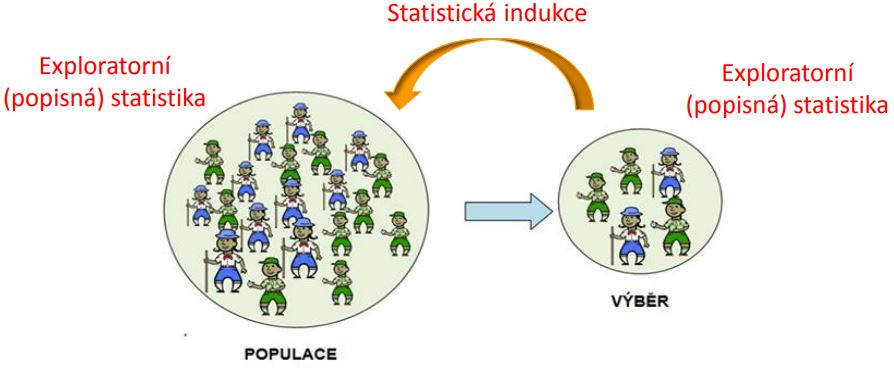
\includegraphics[width=0.6\textwidth]{assets/14_stat_ind}
\end{figure}

\textbf{Základní soubor (populace)}
\begin{itemize}
	\item Je množina všech teoreticky možných objektů (např. jedinců) v uvažované situaci = statistický soubor, který je vymezen cílem výzkumu a pro který vyvozujeme závěry výzkumného šetření.
	\item Charakterizuje se \textbf{parametrem}, což je např. výška, váha, IQ, atp.
	\item Má konečný nebo nekonečný (hypotetický) \textbf{rozsah}, který je dán N (např.: N = 150 lidí, opic, rostlin,...).
\end{itemize}
\textbf{Výběrový soubor (výběr)}
\begin{itemize}
	\item Je část populace vybrané na základě předem stanovených kritérii resp. pravidel (podmnožina základního souboru).
	\item \textbf{O náhodném výběru} uvažujeme, když splňuje dvě základní vlastnosti: pravděpodobnost zařazení do vzorku je pro všechny statistické jednotky populace nenulová a statistické jednotky jsou do vzorku vybrané nezávisle jedna od druhé.
	\item \textbf{O reprezentativním výběru} uvažujeme, když výběrový soubor dobře odráží strukturu celého zkoumaného souboru.
\end{itemize}
\textbf{Principy statistického usuzování}
\begin{enumerate}
	\item Statistické usuzování znamená zobecňování z výběrových statistik na parametry rozdělení.
	\item Abychom mohli provést statistické usuzování, musíme mít nějakou teorii, jež popisuje náhodné chování sledovaných proměnných.
	\item Existují dva typy výběrových chyb: náhodné výběrové chyby a systematické chyby. Získáním náhodného výběru zmenšujeme systematickou chybu a získáváme podklad pro odhad náhodné výběrové chyby.
	\item Výběrová rozdělení statistik jsou teoretická pravděpodobnostní rozdělení, která popisují vztah mezi výběrovou statistikou a populací.
	\item Směrodatná odchylka výběrového rozdělení statistiky (odhad parametru) se nazývá směrodatná chyba. Odhaduje náhodnou výběrovou chybu vypočítané statistiky (odhadu parametru).
	\item Jak roste velikost výběru, výběrová chyba a směrodatná chyba se zmenšují.
	\item Směrodatná chyba se používá k získání intervalového odhadu parametrů i k testování hypotéz o parametrech rozdělení.
\end{enumerate}

\subsubsection{Intervalové odhady}
\begin{itemize}
\item V praktických aplikacích často určujeme \textbf{odhad příslušného parametru} pomocí intervalového odhadu.
\item Tento odhad je reprezentován intervalem $<t_D, t_H>$, v němž hledaný parametr leží s předem určenou pravděpodobností (spolehlivostí), kterou označujeme $(1 − \alpha)$.
\item neboli parametr populace aproximujeme intervalem, v němž s velkou pravděpodobností příslušný populační parametr leží.
\end{itemize}

\begin{itemize}
	\item \textbf{Interval spolehlivosti}(konfidenční interval) pro parametr $\theta$ se spolehlivostí $1−\alpha$,kde $\alpha \in <0; 1>$ , je taková dvojice statistik $(T_D, T_H)$, že $P(T_D \leq \theta \leq T_H) = 1 − \alpha$.
\end{itemize}
\begin{figure}[H]
\centering
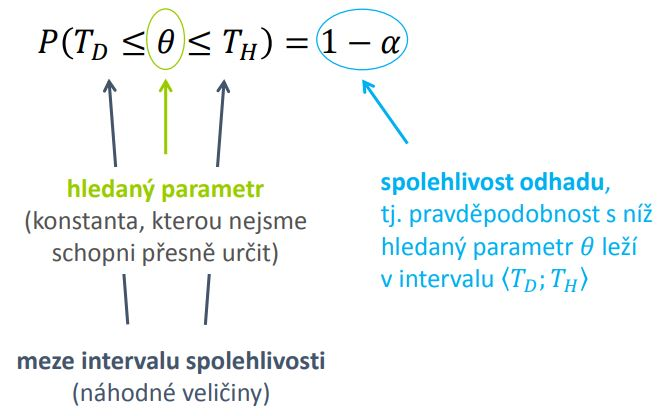
\includegraphics[width=0.6\textwidth]{assets/14_inter_odhad_terminologie}
\end{figure}
\begin{itemize}
	\item \textbf{Intervalový odhad} $t_D,t_H$ je jednou z realizací intervalu spolehlivosti.
	\item Požadavky na interval spolehlivosti:
	\begin{itemize}
		\item Co \textbf{největší spolehlivost} odhadu.
		\item Co \textbf{nejmenší šírka} intervalu spolehlivost. (S rostoucí šířkou intervalového odhadu klesá významnost získané informace.)
	\end{itemize}
	\item S rostoucí spolehlivostí se zvětšuje šířka intervalového odhadu a tím klesá významnost takto získané informace.
	\item S rostoucím rozsahem výběru se šíčka intervalového odhadu snižuje.
	\item Typy intervalů spolehlivosti:
	\begin{itemize}
		\item \textbf{oboustranné} 
		\begin{equation*}
				P(\theta < T_D) = P(\theta > T_H) = \frac{\alpha}{2}
		\end{equation*}
		Tyto dvě podmínky zaručují, že $P(T_D \leq \theta \leq T_H) = 1 - \alpha$
		\item \textbf{jednostranné} (odhadujeme--li například délku života nějakého zařízení, je pro nás důležitá pouze dolní mez)
		\begin{itemize}
			\item \textbf{levostranné} $P(\theta \geq T_D^*) = 1 - \alpha$
			\item \textbf{pravostranné} $P(\theta \leq T_H^*) = 1 - \alpha$
		\end{itemize}
	\end{itemize}
\end{itemize}
\begin{figure}[H]
\centering
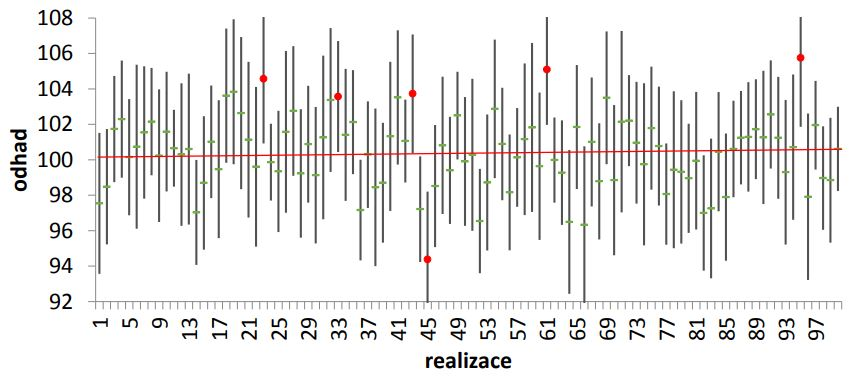
\includegraphics[width=0.6\textwidth]{assets/14_spolehlivost_odhadu}
\caption{Co to znamená, že spolehlivost odhadu je $1- \alpha$? \\Simulace 100 intervalových odhadů střední hodnoty (spolehlivost $0,95$) získaných na základě opakovaných výběrů o rozsahu 30 z populace se střední hodnotou 100. 6 intervalů ze 100 neobsahuje skutečnou střední hodnou}
\end{figure}
\subsection{Jak najít intervalový odhad parametru $\theta$?}
\textbf{Obecně:}
\begin{enumerate}
	\item Zvolíme vhodnou výběrovou charakteristiku $T(\mathbf{X})$, jejíž rozdělení známe.
	\item \begin{equation*}
			\begin{split}
				P(\frac{x_\alpha}{2} \leq T(\mathbf{X}) \leq x_{1 - \frac{alpha}{2}}) = 1 - \alpha, \\
				P(T(\mathbf{X}) \leq x_{1-\alpha}) = 1 - \alpha, \\
				P(T(\mathbf{X}) \geq x_\alpha) = 1 - \alpha.	
			\end{split}
		\end{equation*}
\end{enumerate}